% -*- coding: utf-8 -*-

\chapter{プログラマ的同人誌執筆環境構築概論}
% * (アスタリスク)付きの \chapter* コマンドは原則不可とする

\begin{flushright}
 はやみず
\end{flushright}

\lettrine{技}
術者たるもの、同人誌を書く時であってもその技術的ノウハウを積極的に投入し
て、執筆作業を最大限に効率化しなければならない。そのような信条のもとに、
本誌の執筆環境は構築された。

% \vspace*{2mm}
% 
% \begin{center}
%  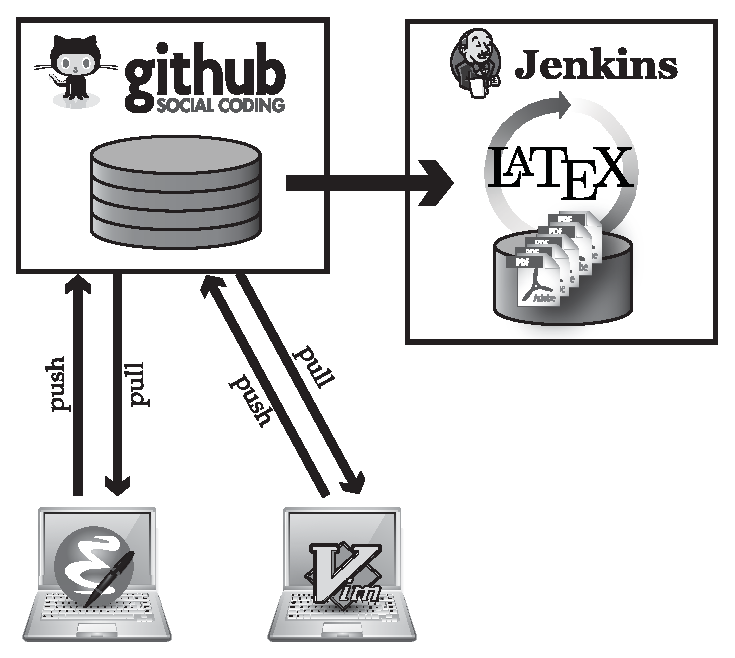
\includegraphics[width=8cm]{hayamiz/images/dbtimes-env.eps}
% \end{center}

\section{LaTeX}

文章執筆はLaTeXに限る。

% 文章ファイルの保存形式は、やはりプレインテキストでなければならない。最近
% はWordも構造化された文章を執筆するための機能が整いつつあるという。しかし
% ながら、我々はプログラマである。プログラマは、各自の研ぎ澄まされたテキス
% トエディタ環境を有している。即ち、執筆速度を最大化するためには、各々が最
% 大限能力を発揮できるテキストエディタ環境を利活用することが最善である。そ
% のためには、やはりプレインテキストでなければならない。

文章ファイルの保存形式は、やはりプレインテキストでなければならない。プロ
グラマは各自の研ぎ澄まされたテキストエディタ環境を有している。即ち、執
筆速度を最大化するためには、各々が最大限能力を発揮できるテキストエディタ
環境を利活用することが最善である。そのためには、やはりプレインテキストで
なければならない。

そして、我々プログラマは情報を構造化されていない状況に極度のストレスを覚
える生き物である。ある程度以上の長さ、内容の高度さをもつ文章を執筆する場
合には、図表や章・節の参照、文献管理、目次の作成、整合性のある文章スタイ
ル調整など、文章全体が高度に構造化され、文章内の要素が有機的に結合されて
いなければならない。これを為すためには、高度かつ柔軟な組版システムを利用
することが必要不可欠である。

やはり、文章執筆はLaTeXに限る。

本誌の組版には \TeX Live 2011 を用いてる。文書のクラスには奥村先生の
{\tt jsbook.cls} を利用しており、{\tt tombow} オプションを利用することで
トンボ付きの出力を得ている。{\tt tombow}オプションを利用する際には、併せ
て{\tt papersize}オプションを利用しないと、文書のサイズとしてはトンボ無し
で出力されてしまうので注意が必要である。

\section{GitHub}

文章執筆はGitHubに限る。

複数名で共同作業を行う場合、最近では Dropbox が用いられる場合が多い。
Dropbox は便利である。一度導入してしまえば、誰でも簡単にファイルを即時に
共有することができる。

しかし、我々はプログラマである。プログラマは変更履歴を重んじる生き物であ
る。即ち、バージョン管理システムはプログラマにとって必須である。Dropboxに
も履歴管理機能は存在するが、限定的でありインターフェースも非効率なもので
ある。

また、プログラマは編集の競合に注意を払う生き物である。特に本誌のように締
切のあるようなものの場合、締切直前には多数の編集が競合することが予想され
る。Dropbox では、競合の解決をシステマティックに行うことは不可能である。
一方、バージョン管理システムはその基本機能として競合解決のシステマティッ
クな方法を提供する。バージョン管理システムに高いリテラシを有する我々にとっ
て、これを用いないことは有り得ない。

そして今日、GitHubはプログラマの共通基盤である。殆どのプログラマは、各々
のSSH公開鍵をGitHubに登録済みである。即ち、GitHubをバージョン管理システム
のホストとして用いることで、最小限の手間で共同作業基盤を構築可能である。

幸いなことに、私はGitHubのプライベートレポジトリを作成できるアカウントを
保有している。そのため、原稿はクローズドな形で管理することが可能である。

やはり、文章執筆はGitHubに限る。

\section{継続的インテグレーション}

文章執筆は継続的インテグレーションに限る。

我々は重要な事実に目を向けなければならない。\LaTeX の基盤たる \TeX という
言語は、単なるマークアップ言語にあらず。チューリング完全性を有する、完備
なるプログラミング言語であり、\LaTeX による文章執筆とは即ちプログラミン
グ行為であり、ソフトウェア開発にほかならないのである。

ソフトウェア開発において、今日最も重要視されている開発基盤の一つが継続的
インテグレーションである。バージョン管理システムにコードがコミットされる
度に、プログラムがビルドされ、テストコードが走り、常に最新の成果物が生成
された状態が維持される。一度誤ったコードがコミットされた折には、そのこと
が開発者に直ちに通知され、更なる状況の悪化を食い止めるフィードバックルー
プを形成する。

% また、\LaTeX による文章執筆における特有の問題として、最終成果物であるPDF
% ファイルに正しくフォントを埋め込むための環境構築には一定の手間を要すると
% いうことがある。執筆者全員が、あまねく必要なフォントをすべて保持し、適切
% に \LaTeX 環境を設定することは難しい。必要なフォントを持たない場合には、
% 代替フォントによって文章をプレビューする他にない。一方で、継続的インテグ
% レーションのためのビルドサーバにおいてこのような環境を構築しておけば、執
% 筆者全員が最終成果物を正しい形で確認することが可能である。

本誌の執筆においては、継続的インテグレーションシステムJenkinsを導入し、
GitHubのコミットにフックしてPDFファイルの生成を行うことにより、即座に入稿
可能な状態の原稿が常に確認可能な環境を構築した。

やはり、文章執筆は継続的インテグレーションに限る。